\chapter{實驗結果}
\label{章:實驗結果}

\begin{table}
\caption{實驗工具版本}
\label{表:實驗工具版本}
\centering
\begin{tabular}{l|l}
工具 & 版本\\
\hline
臺灣言語工具\cite{臺灣言語工具} & 0.5.0\\
Moses\cite{Koehn:2007:MOS:1557769.1557821} & commit 40c819d285cdeb40c0b8cc428bfde2fcb531b655\\
GIZA++\cite{och2003systematic} & 1.0.7\\
SRILM\cite{stolcke2002srilm} & 1.7.0\\
\end{tabular}
\end{table}

為著逐家後壁研究的方便,
本論文研究的程式佮結果,
全部公開佇網路頂的專案\cite{翻譯研究}。
開發工具的版本會當看表\ref{表:實驗工具版本},
詳細的參數,
可比講語言模型用Witten-Bell加discounting的算法,
翻譯模型用預設的訓練包攏會當佇內底的設定看著。
\section{閩南語詞實驗}
\label{節:閩南語詞實驗}

\begin{table}
\caption{閩南語詞的效果}
\label{表:閩南語詞的效果}
\centering
\begin{tabular}{c|ccc}
斷詞方法 & 召回率 & 精確率 & F測量\\
\hline
拄好長度斷詞 & 91.1 & 85.1 & 88.0\\
長詞優先斷詞(對頭前) & 91.0 & 84.9 & 87.9\\
長詞優先斷詞(對後壁) & 91.1 & 85.0 & 88.0\\
\end{tabular}
\end{table}

本實驗是提教育部辭典的35130个詞條當做訓練語料,
試驗語料是教育部辭典例句8027句。
共試驗語料的斷詞資訊提掉了後,
用拄好長度斷詞佮長詞優先去斷詞,
才閣佮原本例句的斷詞比較,
得著表\ref{表:閩南語詞的效果}的結果。

會當看著拄好長度斷詞的分數有比長詞優先閣較好淡薄,
毋過無明顯的進步。
這兩種斷詞方法的精確率攏比召回率低誠濟,
代表辭典內底收的詞閣無夠濟。

\section{語料整理實驗}
\label{節:語料整理實驗}

\begin{figure}
\centerline{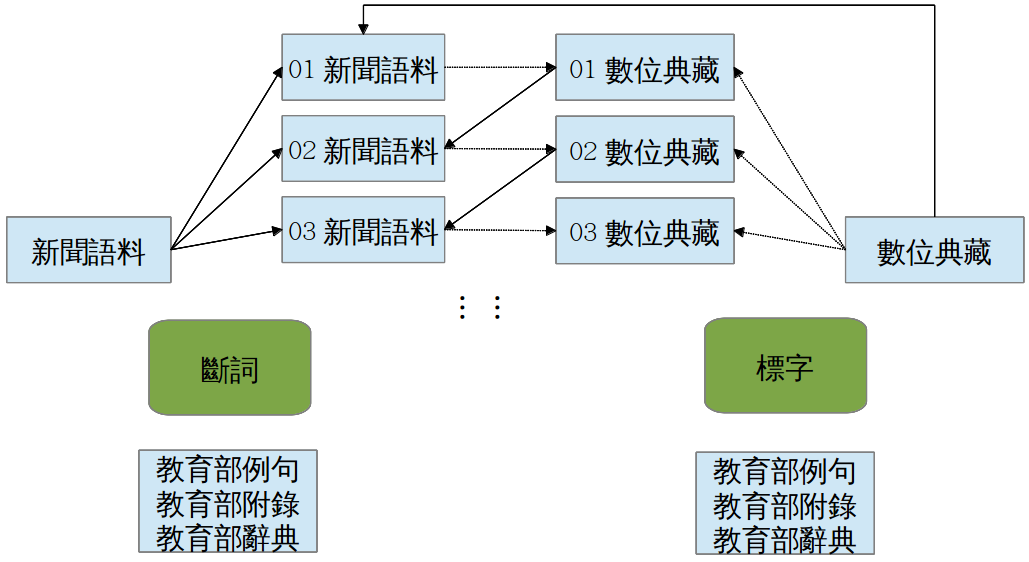
\includegraphics[keepaspectratio,width=40em]{圖/互相整理架構}}
\caption{互相整理流程}
\label{圖:互相整理架構}
\end{figure}

\begin{table}
\caption{新聞語料庫佮數位典藏互相整理的實驗}
\label{表:互相整理實驗}
\centering
\begin{tabular}{lcccccc}
整理幾擺 & 原始語料 & 1 & 2 & 3 & 4 & 5\\
BLEU分數 & 9.30 & 14.72 & 13.77 & 13.82 & 13.82 & 13.82\\
\end{tabular}
\end{table}



完整的閩南語語料愛有全漢、全羅佮斷詞資訊。
因為新聞語料庫有全漢、全羅,無斷詞,數位典藏有斷詞毋過無完整的全漢佮全羅。
%做表

%,教育部辭典斷詞佮全漢全羅攏有。
%攏就會使用教育部辭典佮數位典藏共新聞語料庫斷詞,閣共斷好的新聞語料庫佮教育部辭典提來標數位典藏的一對一,閣重做幾仔擺,到收斂為止,親像圖XX。

本實驗是提教育部辭典的35130个詞條佮附錄388句當做標準語料,
用拄好長度斷詞來整理新聞平行語料64121句佮數位典藏329476句。
因為逐个資料庫有的資訊攏無仝,
會使做親像圖\ref{圖:互相整理架構}一樣做誠濟擺的整理。

%頂一章使用新聞語料庫,語言模型嘛是用平行語料的閩南語訓練的,其實這馬有一大部份的閩南語語料攏毋是平行話料,攏是純閩南語一種語言爾爾。
%這種純閩南語的語料其實嘛會當提來訓練語言模型,毋過語料的形式就有足濟款的,親像有漢羅、全羅佮全漢等等。有的語料會敆兩種以上的文本。來互相整理,翻譯的效果閣較好。
%毋過語料的形式無仝,會當利用的部份就無仝。親像全羅會當提供斷詞的資訊,有漢字佮拼音一對一的當提來做辭典。
%這章會加入新的語料庫,而且利用⿰因無仝款的性質,

表\ref{表:互相整理實驗}是整理的結果,
分數是用詞為單位拍的。
整理的結果一息仔就收斂,
會當看著整理了的分數比猶未整理前好欲一半。
毋過整理第二擺了後,分數有降一寡,
看整理了的結果,
是因為新聞佮典藏內底的攏有一寡錯誤,
所以第二擺用著遮的資料,
會影響著整理的結果。

%人-為|jin5-ui5 的|e5
%人-為-的|jin5-ui5-e5


\section{分類語言實驗}
\label{節:判斷語言實驗}

\begin{figure}
\caption{無仝特徵詞數量,分類3741段閩南語華語}
\label{圖:無仝特徵詞數量對分類閩南語華語效果的影響}
\begin{tikzpicture}
\begin{axis}[
scaled y ticks=real:1,
ytick scale label code/.code={},
ymax = 14,
symbolic x coords={0,10,20,50,100,200,500,1000,2000,3000},
xtick=data,
height=8cm,
width=14cm,
grid=major,
xlabel={特徵詞數量},
ylabel={分類錯誤率},
legend style={
cells={anchor=east},
legend pos=north east,
%mark size=0.5em
}
]
\addplot coordinates {
(0,13.79) (10,6.87) (20,5.45) (50,4.12)
(100,3.88) (200,3.90) (500,4.12)
(1000,3.80) (2000,4.14) (3000,4.14)
%(0,516) (10,257) (20,204) (50,154)
%(100,145) (200,146) (500,154)
%(1000,142) (2000,155) (3000,155)
};

\legend{SVM}
\end{axis}
\end{tikzpicture}
\end{figure}

%n=7000,m=3000
%選特徵詞的方法是先統計的試驗語料佮數位典藏,
%揀出頭前n个上定出現的閩南語定用詞\footnote{有標點符號}
%華語部份嘛仝款,佇中央研究院現代漢語標記語料庫\footnote{\url{http://app.sinica.edu.tw/cgi-bin/kiwi/mkiwi/kiwi.sh}}內底揣n个上定出現的華語定用詞,
%閣來對上定用的閩南語定用詞開始,若這个定用詞的漢字詞無出現佇華語15000定用詞內底,就共伊當做特徵詞。


%有閩南語佮華語的特徵詞了後,咱對網頁整理出一段一段的語料,先用\ref{節:拄好長度斷詞}節的閩南語詞,看斷詞出來的結果,佇閩南語7000个特徵出中,分別出現幾个。
%除了7000个特徵詞,咱閣用閩南語語言模型分數,斷詞了的全部詞數,1~4字詞分別數量\footnote{「我 想 欲 食飯」就有3个一字詞,1个兩字詞,全部4个詞},按呢干焦閩南語就有7006个特徵,摻華語就有14012个特徵。


這節實驗的語料是對TGB通訊創刊開始,到2014年6月12日為止攏總177期1179篇文章,
提出頭前1000篇做訓練語料,閩南語有9368段488844詞,華語有8519段439436詞;
後壁179篇做訓練語料,閩南語有1344段75282詞,華語有2397段114901詞。
以段做辨識單位,提來予支援向量機分類。

毋過6012个特徵實在是傷濟矣,所以咱試看覓共3000特徵詞減少,看會影響著辨識率無。
實驗結果佇表\ref{圖:無仝特徵詞數量對分類閩南語華語效果的影響},
佇50~100个特徵詞分類效果就收斂矣,加閣較濟的特徵詞,無啥影響著辨識的效果。

\section{加入TGB語料庫實驗}
\label{節:加入TGB語料庫實驗}

\begin{table}
\caption{加入TGB語料的翻譯效果}
\label{表:加入TGB語料的翻譯效果}
\centering
\begin{tabular}{lcccccc}
& 加TGB語料前 & 加TGB語料後\\
平行語料句數 & 64121句 & 99146句\\
BLEU分數 & 13.82 & 19.33\\
\end{tabular}
\end{table}

頂一節做分類語言的實驗,
紲落來就是共TGB語料摻入來翻譯語料。

先提教育部詞條佮附錄句和
\ref{節:語料整理實驗}節整理了的新聞佮典藏語料
來整理TGB語料,
閣用Bleualign來對齊,
就會使提著35025句TGB平行語料。

實驗訓練語料除了\ref{節:語料整理實驗}節的語料外,
閣加入TGB平行語料,
除了教育部附錄句、典藏干焦會使做語言模型以外,
原本平行語料干焦是新聞語料庫64121句,
加入TGB語料35025句了後變做99146句,
對表\ref{表:加入TGB語料的翻譯效果}會當看著進步誠濟,
代表平行語料閣無夠,
閣佇加語料就會使幫助翻譯的階段。
%母語愛專注佇語料處理

\section{斷詞樣式佮斷字樣式的翻譯結果實驗}
\label{節:斷詞樣式佮斷字樣式的翻譯結果實驗}


\begin{figure}
\caption{斷字佮斷詞語料的翻譯效果比較ーBLEU用詞拍分數}
\label{圖:斷字佮斷詞語料的翻譯效果比較ーBLEU用詞拍分數}
\begin{tikzpicture}
    \begin{axis}[
        width  = 0.85*\textwidth,
        height = 8cm,
        major x tick style = transparent,
        x tick label style={rotate=30,anchor=east},
        ybar=2*\pgflinewidth,
        bar width=14pt,
        ymajorgrids = true,
        ylabel = {BLEU分數},
        symbolic x coords={華語斷字-閩南語字,華語斷字-閩南語詞,華語詞-閩南語字,華語詞-閩南語詞},
        xtick = data,
        enlarge x limits=0.25,
		legend pos=north west,
    ]
        \addplot
            coordinates {(華語斷字-閩南語字, 10.60) (華語斷字-閩南語詞,17.96)
  	          (華語詞-閩南語字,10.62) (華語詞-閩南語詞,18.64)};
        \addplot
            coordinates {(華語斷字-閩南語字, 10.60) (華語斷字-閩南語詞,17.96)
  	          (華語詞-閩南語字,11.06) (華語詞-閩南語詞,19.33)};
        \addplot
            coordinates {(華語斷字-閩南語字, 10.60) (華語斷字-閩南語詞,17.96)
  	          (華語詞-閩南語字,10.83) (華語詞-閩南語詞,19.13)};
        \legend{無處理未知詞,華字-閩字翻譯,華字-閩詞翻譯}
    \end{axis}
\end{tikzpicture}
\end{figure}

\begin{figure}
\caption{斷字佮斷詞語料的翻譯效果比較ーBLEU用字拍分數}
\label{圖:斷字佮斷詞語料的翻譯效果比較ーBLEU用字拍分數}
\begin{tikzpicture}
    \begin{axis}[
        width  = 0.85*\textwidth,
        height = 8cm,
        major x tick style = transparent,
        x tick label style={rotate=30,anchor=east},
        ybar=2*\pgflinewidth,
        bar width=14pt,
        ymajorgrids = true,
        ylabel = {BLEU分數},
        symbolic x coords={華語字-閩南語字,華語字-閩南語詞,華語詞-閩南語字,華語詞-閩南語詞},
        xtick = data,
        enlarge x limits=0.25,
		legend pos=north east,
    ]
        \addplot
            coordinates {(華語字-閩南語字, 31.85) (華語字-閩南語詞,31.24)
  	          (華語詞-閩南語字,30.74) (華語詞-閩南語詞,29.22)};
        \addplot
            coordinates {(華語字-閩南語字, 31.85) (華語字-閩南語詞,31.26)
  	          (華語詞-閩南語字,31.90) (華語詞-閩南語詞,30.92)};
        \addplot
            coordinates {(華語字-閩南語字, 31.85) (華語字-閩南語詞,31.24)
  	          (華語詞-閩南語字,31.44) (華語詞-閩南語詞,30.43)};
        \legend{無處理未知詞,華字-閩字翻譯,華字-閩詞翻譯}
    \end{axis}
\end{tikzpicture}
\end{figure}

為著愛無仝形式的語料對翻譯效果的影響,
就共全部的狀況試一擺。
華語佮閩南語兩種語言,
摻字佮詞兩種形式,
攏總有「華語字-閩南語字」、「華語字-閩南語詞」、
「華語詞-閩南語字」,「華語詞-閩南語詞」四个狀況。

因為華語拿用詞做單位,
會出現節的未知詞問題,
若翻譯袂出來,
就用「華語字-閩南語字」抑是「華語字-閩南語詞」的翻譯模型去處理,
結果會當看圖\ref{圖:斷字佮斷詞語料的翻譯效果比較ーBLEU用詞拍分數},
這个實驗的訓練、試驗語料佮頂一个實驗是仝款的。

因為上尾比較是用詞做單位,
所以「華語字-閩南語字」佮「華語詞-閩南語字」的結果愛閣重斷工,
會當看著「華語詞-閩南語詞」的翻譯效果上好,
毋閣若用字做單位,
佇圖\ref{圖:斷字佮斷詞語料的翻譯效果比較ーBLEU用字拍分數}的實驗,
「華語字-閩南語詞」分數上懸。

這个實驗會當看著幾件代誌,
第一个是用詞拍分數的情形下「華語詞-閩南語詞」效果上好,
因為翻譯了的文本若需要語音合成抑是再利用,
攏需要斷詞的資訊,
代表講用「華語字-閩南語詞」是上好的。
雖然用字做單位拍分數時伊分數毋是上懸,
毋過別的組合需要重斷詞,
會當看著重斷詞影響著上尾的分數誠濟。

第二个是未知詞若有處理,
對翻譯有幫助,
而且未知詞用「華語字-閩南語字」的效果比「華語字-閩南語詞」閣較好,
可能是因為未知詞大部份攏是需要一字一字照翻的,
嘛有可能是語料無夠濟,
斷字對斷字的統計數量較濟。

上尾第三件代誌是華語的斷詞對翻譯有幫助,
毋過閩南語的斷詞煞無。
可能是閩南語的斷詞閣無夠準,
造成翻譯效果變\ji{⿰禾黑}。
